% This is samplepaper.tex, a sample chapter demonstrating the
% LLNCS macro package for Springer Computer Science proceedings;
% Version 2.21 of 2022/01/12
%
\documentclass[runningheads]{llncs}
%
\usepackage[T1]{fontenc}
% T1 fonts will be used to generate the final print and online PDFs,
% so please use T1 fonts in your manuscript whenever possible.
% Other font encondings may result in incorrect characters.
%
\usepackage{graphicx}
% Used for displaying a sample figure. If possible, figure files should
% be included in EPS format.
%
% If you use the hyperref package, please uncomment the following two lines
% to display URLs in blue roman font according to Springer's eBook style:
% \usepackage{color}
% \renewcommand\UrlFont{\color{blue}\rmfamily}
%
\usepackage{hyperref}
\usepackage{paralist}
\usepackage{booktabs}
\usepackage{totcount}
\usepackage{amssymb}

\newcounter{totHours} %to track the estimate of total hours to assess SOP
\setcounter{totHours}{0}
\regtotcounter{totHours}

\newcounter{rqnum} %research question number
\newcommand{\rqtherqnum}{RQ`'\therqnum}
\newcommand{\rqref}[1]{RQ\ref{#1}}

\newcounter{pnum} %pain point number
\newcommand{\ppthepnum}{P`'\thepnum}
\newcommand{\ppref}[1]{P\ref{#1}}

\newcommand{\CC}{C\nolinebreak\hspace{-.05em}\raisebox{.4ex}{\small\bf
+}\nolinebreak\hspace{-.10em}\raisebox{.4ex}{\small\bf +}}

\begin{document}
%
% \title{Digging Deep to Assess the State of the Practice for Different Research Software Domains}
\title{Digging Deeper Into the State of the Practice for Domain Specific Research Software}
\titlerunning{Digging Deeper}
% If the paper title is too long for the running head, you can set
% an abbreviated paper title here
%
\author{Spencer Smith\inst{1}\orcidID{0000-0002-0760-0987} \and
Peter Michalski\inst{1}}%\orcidID{1111-2222-3333-4444} \and
%Third Author\inst{3}\orcidID{2222--3333-4444-5555}}
%
\authorrunning{S.\ Smith and P.\ Michalski}
% First names are abbreviated in the running head.
% If there are more than two authors, 'et al.' is used.
%
\institute{McMaster University, 1280 Main Street West, Hamilton ON L8S 4K1, Canada
\email{smiths@mcmaster.ca}\\
\url{http://www.cas.mcmaster.ca/~smiths/}}
%
\maketitle              % typeset the header of the contribution
%
\begin{abstract}

	To improve software development methods and tools for research software, we
	first need to understand the current state of the practice.  Therefore, we
	have developed a methodology for assessing the state of the software
	development practices for a given research software domain.  The methodology
	is applied to one domain at a time in recognition that software development in
	different domains is likely to have adopted different best practices.
	Moreover, providing a means to measure different domains facilitates
	comparison of development practices between domains.  For each domain we wish
	to answer questions such as: 
  \begin{inparaenum}[i)]
    \item What artifacts (documents, code, test cases, etc.) are present?
    \item What tools are used?
    \item What principles, process and methodologies are used?
    \item What are the pain points for developers?
    \item What actions are used to improve qualities like maintainability and
    reproducibility?
  \end{inparaenum} 
  To answer these questions, our methodology prescribes the following steps: 
  The abstract should briefly summarize the contents of the paper in 150--250 words.

\keywords{First keyword  \and Second keyword \and Another keyword.}
\end{abstract}

\section{Introduction} \label{SecIntroduction}

Research software is critical for tackling problems in areas as diverse as
manufacturing, financial planning, environmental policy and medical diagnosis
and treatment.  However, developing reliable, reproducible, sustainable and fast
research software to address new problems is challenging because of the
complexity of the physical models and the nuances of floating point and parallel
computation. The importance of research software and the difficulty with its
development have prompted multiple researchers to investigate how developing
this software differs from other classes of software.  Previous studies have
focused on surveying developers \cite{Carveretc}, developer interviews \cite{}
and case studies \cite{Segal}.  A valuable source of information that has
received less attention is the data in the publicly available software
repositories.  We propose a new methodology for digging deeper into how well
projects are applying best practices by using a combination of manual and
automated techniques to extract repository-based information.

The surveys used in previous studies have tended to recruit participants from
all domains of research software, possibly distinguishing them by programming
language (for instance, R developers \cite{Rstudy}), or by the role of the
developers (for instance postdoctoral researchers \cite{Katz}).  For their part,
case studies have focused on a few specific examples at a time, since that is
the nature of case studies.  We propose applying our new methodology between
these two extremes.  Rather than focus on all research software, or just a few
examples, we will focus on one domain of research software at a time. The
practical reason for defining a domain scope is that digging deep into
repository data takes time, making a broad scope infeasible.  We have the
constraint that the work load for applying the methodology to a given domain
needs to be feasible for a team as small as one individual, and for a time that
is short, ideally around a person month per domain.\footnote{A person month is
considered to be $20$ working days ($4$ weeks in a month, with $5$ days of work
per week) at $8$ person hours per day, or $20 \cdot 8 = 160$ person hours.}
Focusing on one domain at a time has more than just practical advantages.  By
restricting ourselves to a single domain we can bring domain knowledge and
domain experts into the mix.  The domain customized insight provided by the
assessment has the potential to help a specific domain as they adopt and develop
new development practices.  Moreover, providing a means to measure different
domains facilitates uncovering domain specific practices, which can later be
compared and contrasted between different domains.

Our methodology is built around 10 research questions for the domain being
assessed.  The questions are used to structure the presentation of the
methodology, so for each research question we point to the corresponding section
of the paper.  Assuming we have identified the domain of interest, the first question is:

\begin{enumerate}
	\item[RQ\refstepcounter{rqnum}\therqnum \label{RQ_WhatProjects}:] What
	software projects exist in the domain, with the constraint that the source
	code must be available for all identified projects?
	(Section~\ref{methodology})
\end{enumerate}

We next wish to assess the representative software to determine how well they
apply current software development best practices.  At this point in the
process, to remove potential user/developer bias, we will base our assessment
only on publicly available artifacts, where artifacts are the documents, scripts
and code that we find in a project's public repository. Example artifacts
include requirements, specifications, user manuals, unit test cases, system
tests, usability tests, build scripts, API (Application Programming Interface)
documentation, READMEs, license documents, process documents, and code.
Following best practices does not guarantee popularity, so we will also compare
our ranking to how the user community itself ranks the identified projects.

\begin{enumerate}
	\item [RQ\refstepcounter{rqnum}\therqnum \label{RQ_HighestQuality}:] Which
	of the projects identified in \rqref{RQ_WhatProjects} follow current best
	practices, based on evidence found by experimenting with the software and
	searching the artifacts available in each project's repository? (Section~\ref{AHPresults})
	\item [RQ\refstepcounter{rqnum}\therqnum \label{RQ_CompareHQ2Popular}:] How
	similar is the list of top projects identified in \rqref{RQ_HighestQuality}
	to the most popular projects, as viewed by the scientific community? (Section~\ref{repmetrics})
\end{enumerate}

To understand the state of the practice we wish to learn the frequency with
which different artifacts appear, the types of development tools used and the
methodologies used for software development.  With this data, we can ask
questions about how the domain software compares to other research software.

\begin{enumerate}
  \item [RQ\refstepcounter{rqnum}\therqnum \label{RQ_CompareArtifacts}:] How
	do domain projects compare to research software in general with respect to the
	artifacts present in their repositories? (Section~\ref{Sec_CompareArtifacts})
	\item [RQ\refstepcounter{rqnum}\therqnum \label{RQ_CompareToolsProjMngmnt}:]
	How do domain projects compare to research software in general with respect to
	the use of tools (Section~\ref{Sec_CompareTools}) for:
	\begin{enumerate} 
		\item [\rqref{RQ_CompareToolsProjMngmnt}.a] development; and,
		\item [\rqref{RQ_CompareToolsProjMngmnt}.b] project management?
	\end{enumerate}
	\item [RQ\refstepcounter{rqnum}\therqnum \label{RQ_CompareMethodologies}:]
	How do domain projects compare to research software in general with respect to
	principles, processes and methodologies used? (Section~\ref{Sec_CompareMethodologies})
\end{enumerate}	

Only so much information can be gleaned by digging into software repositories.
To gain additional insight, we need to interview developers.  We need to learn
their concerns and how they deal with these concerns; we need to learn their
pain points.  We wish to know what practices are used by the top domain
projects, so that others can potentially emulate these practices. We also wish
to identify new practices by borrowing successful ideas from other domains. The
above points are covered by the questions outlined below:

\begin{enumerate}
	\item [RQ\refstepcounter{rqnum}\therqnum \label{RQ_PainPoints}:] What are
	the pain points for developers working on domain software projects?
	(Section~\ref{painpoints})
	\item [RQ\refstepcounter{rqnum}\therqnum \label{RQ_ComparePainPoints}:] How
	do the pain points of domain developers compare to the pain points
	for research software in general? (Section~\ref{painpoints})
	\item [RQ\refstepcounter{rqnum}\therqnum \label{RQ_Concerns}:] For domain
	developers what specific best practices are taken to address the pain points
	and software quality concerns? (Section~\ref{Sec_AddressConcerns})
	\item [RQ\refstepcounter{rqnum}\therqnum \label{RQ_Recommend}:]
	What research software development practice could potentially address the
	pain points identified in \rqref{RQ_PainPoints}).
	(Section~\ref{Sec_Recommendations})
\end{enumerate}

Our methodology answers the research question through inspecting repositories,
using the Analytic Hierarch Process (AHP) for ranking software, interviewing
developers and interacting with at least one domain expert.  We leave the
measurement of the performance, for instance using benchmarks, to other projects
\cite{kaagstrom1998gemm}. The current methodology updates the approach used in
prior assessments of domains like Geographic Information Systems
\cite{SmithEtAl2018_arXivGIS}, Mesh Generators \cite{SmithEtAl2016}, Seismology
software \cite{SmithEtAl2018}, and statistical software for psychology
\cite{SmithEtAl2018_StatSoft}.  Initial tests of the new methodology have been
done for medical image analysis software \cite{Dong2021} and for Lattice
Boltzmann Method (LBM) software \cite{Michalski2021}.  The LBM example will be
used throughout this paper to illustrate the steps in the methodology.  The
paper ends with a summary of potential threats to validity
(Section~\ref{threats}) and our final conclusions and recommendations
(Section~\ref{conclusion}).

\section{Methodology} \label{StepsAQDS}

The assessment is conducted via the following steps.  The steps depend on
interaction with a Domain Expert partner, as discussed in
Section~\ref{sec_vet_software_list}.

\begin{enumerate}
  \item Identify the domain of interest. (Section~\ref{SecIdentifyDomain})
	\item List candidate software packages for the domain.
	(Section~\ref{identifysoftware})
	\item Filter the software package list. (Section~\ref{filtersoftware})
	\item Gather the source code and documentation for each software package.
	\item Collect quantitative measures from the project repositories.
	(Section~\ref{empiricalmeasures})
	\item Measure using the measurement template.  The full measurement template
	can be found in \cite{SmithEtAl2021}. (Section~\ref{empiricalmeasures})
	\item Interview the developers. (Section~\ref{SecSurvey})
	\item Use AHP to rank the software packages. (Section~\ref{AHP})
	\item Analyze the results and answer the research questions. (Section~\ref{})
\end{enumerate}

Table~\ref{TabPersonHours} estimates the time required (in person hours) to
complete a state of the practice assessment for a single domain.  The table
assumes that the domain has already been decided and the Domain Expert has been
recruited.  The time spent by the Domain Expert is not included in the numbers
shown in the table, since the amount of time that the domain expert will work
independently of the rest of the assessment team will be small.  Moreover, this
amount of time will vary greatly depending on the preferred work habits of the
Domain Expert.  The table follows the steps outlined above. It is assumed that
the template spreadsheets linked in this document, and the developed AHP tool,
will be employed, rather than developing new tools.  The person hours given are
a rough estimate, based on our experience completing assessments for medical
image analysis software \cite{Dong2021} and for Lattice Boltzmann Method (LBM)
software \cite{Michalski2021}.  The estimate assumes 30 software packages will
be measured; the numbers will need to be adjusted if the total packages changes.
The total number of person hours is \total{totHours} hours.  This is close to
our goal of 1 month of person hours (160 hours).  

\begin{table}[h]
  \caption{Estimated Person Hours for Assessing the State of Practice for Domain
  X} \label{TabPersonHours}
  \centering
  \begin{tabular}{p{12.5cm} l}
    \toprule
    \textbf{Task} & \textbf{Hours} \\
    \midrule

    Initial 1 hour meeting with the Domain Expert plus meeting prep & 5
    \addtocounter{totHours}{5} \\

    Identify broad list of candidate software
    (Section~\ref{SecIdentifyCandSoft}) & 12 \addtocounter{totHours}{12} \\

    Filter software list (Section~\ref{SecInitialFilter}) (10 minutes per
    package) & 5 \addtocounter{totHours}{5} \\

	Review software list with Domain Expert (Section~\ref{SecDomainExpert}) & 2
	\addtocounter{totHours}{2} \\

    Domain analysis (with help of Domain Expert)
    (Section~\ref{SecDomainAnalysis}) & 20 \addtocounter{totHours}{20} \\

	Vet domain analysis with Domain Expert (Section~\ref{SecDomainExpert}) & 3
	\addtocounter{totHours}{3} \\

	Gather source code and documentation for each package (10 minutes per
	package)) & 5 \addtocounter{totHours}{5} \\

    Collect repository based data (Section~\ref{SecEmpiricalMeasures}) (10
    minutes per package) & 5 \addtocounter{totHours}{5} \\

	Measure using measurement template (Section~\ref{SecMeasureTemplate}) (2.5
    hours per repo) & 75 \addtocounter{totHours}{75} \\

    Solicit developers for interviews & 2 \addtocounter{totHours}{2} \\

    Conduct interviews (1.5 hour interviews with 10 developers (30\% recruitment
    rate)) & 15 \addtocounter{totHours}{15} \\

    AHP ranking & 2 \addtocounter{totHours}{2} \\

	Work with Domain Expert to vet AHP ranking & 2 \addtocounter{totHours}{2} \\

    Analyze data and answer research questions & 20 \addtocounter{totHours}{20}\\

    \midrule
    \textbf{Total} & \textbf{\thetotHours} \\
    \bottomrule
  \end{tabular}
  
\end{table}  

\subsection{How to Identify the Domain?} \label{SecIdentifyDomain} 

A domain of research software must be identified to begin the assessment. To be
applicable for the methodology described in this document, the chosen domain
must have the following properties:

\begin{enumerate}
\item The domain must have well-defined and stable theoretical underpinning.  A
  good sign of this is the existence of standard textbooks, preferably
  understandable by an upper year undergraduate student.
\item There must be a community of people studying the domain.
\item The software packages must have open source options.
\item A preliminary search, or discussion with experts, suggests that there will
  be numerous, close to 30, candidate software packages in the domain that
  qualify as `research software'.
\end{enumerate}	

\subsection{How to Identify Candidate Software from the Domain?}
\label{identifysoftware}

To answer~\rqref{RQ_WhatProjects} we needed to identify existing projects. The
candidate software should be found through search engine queries targeting
authoritative lists of software.  Candidate places to search include
\href{https://github.com/} {GitHub} and \href{https://swmath.org/} {swMATH}, as
well as through scholarly articles. The Domain Expert
(Section~\ref{sec_vet_software_list}) should also be engaged in selecting the
candidate software.

The following properties were considered when creating the list and reviewing
the candidate software:

\begin{enumerate}
	\item The software functionality must fall within the identified domain.
	\item The source code must be viewable.
	\item The repository based measures should be available, which implies a
	preference for GitHub-style repositories.
	\item The software cannot be marked as incomplete or in an initial state of
	development.
\end{enumerate}

For the LBM example the initial list had 46 packages \cite{Michalski2021}.

\subsection{How to Filter the Software List?} \label{filtersoftware}

If the list of software is too long (over around 30 packages), then steps need
to be taken to create a more manageable list to answer~\rqref{RQ_WhatProjects}.
The following filters were applied in the priority order listed. Copies of both
the initial and filtered lists, along with the rationale for shortening the
list, should be kept for traceability purposes.

\begin{enumerate}
	\item Scope: Software is removed by narrowing what functionality is
	considered to be within the scope of the domain.
	\item Usage: Software packages were eliminated if their installation
	procedure was missing or not clear and easy to follow.
	\item Age: The older software packages (age being measured by the last date
	when a change was made) were eliminated, except in the cases where an older
	software package appears to be highly recommended and currently in use. (The
	Domain Expert should be consulted on this question as necessary.)
\end{enumerate}

For the third item in the above filter, software packages are characterized as
`alive' if their related documentation had been updated within the last 18
month. Otherwise a package is categorized as `dead'.

For the running example of LBM filtering by scope, usage, and age decreased the
initial list of 46 to a list of 24. Many of the removed packages could not be
tested as there was no installation guide, they were incomplete, source code was
not publicly available, a license was needed, or the project was out of scope or
not up to a standard that would support incorporating them into this
study~\cite{Michalski2021}. Of the remaining packages, some were kept on the
list despite being marked as dead due to their prevalence on authoritative lists
on LBM software and due to their surface excellence.

\subsection{Quantitative Measures} \label{empiricalmeasures}

We rank the projects by how well they follow best practices
(\rqref{RQ_HighestQuality}) via a measurement template, as described in
\cite{SmithEtAl2021}.  For each software package (each column in the template),
we fill-in the rows of the template. This process takes about 2 hours per
package, with a cap of 4 hours. The time constraint is necessary so that the
work load is feasible for a team as small as one, given our aim to cap the
measurement phase at 160 person hours \cite{SmithEtAl2021}.  An excerpt of the
template, in spreadsheet form, is shown in
Figure~\ref{measurement_template_image}.

\begin{figure}[!ht]
	\begin{center}
	  %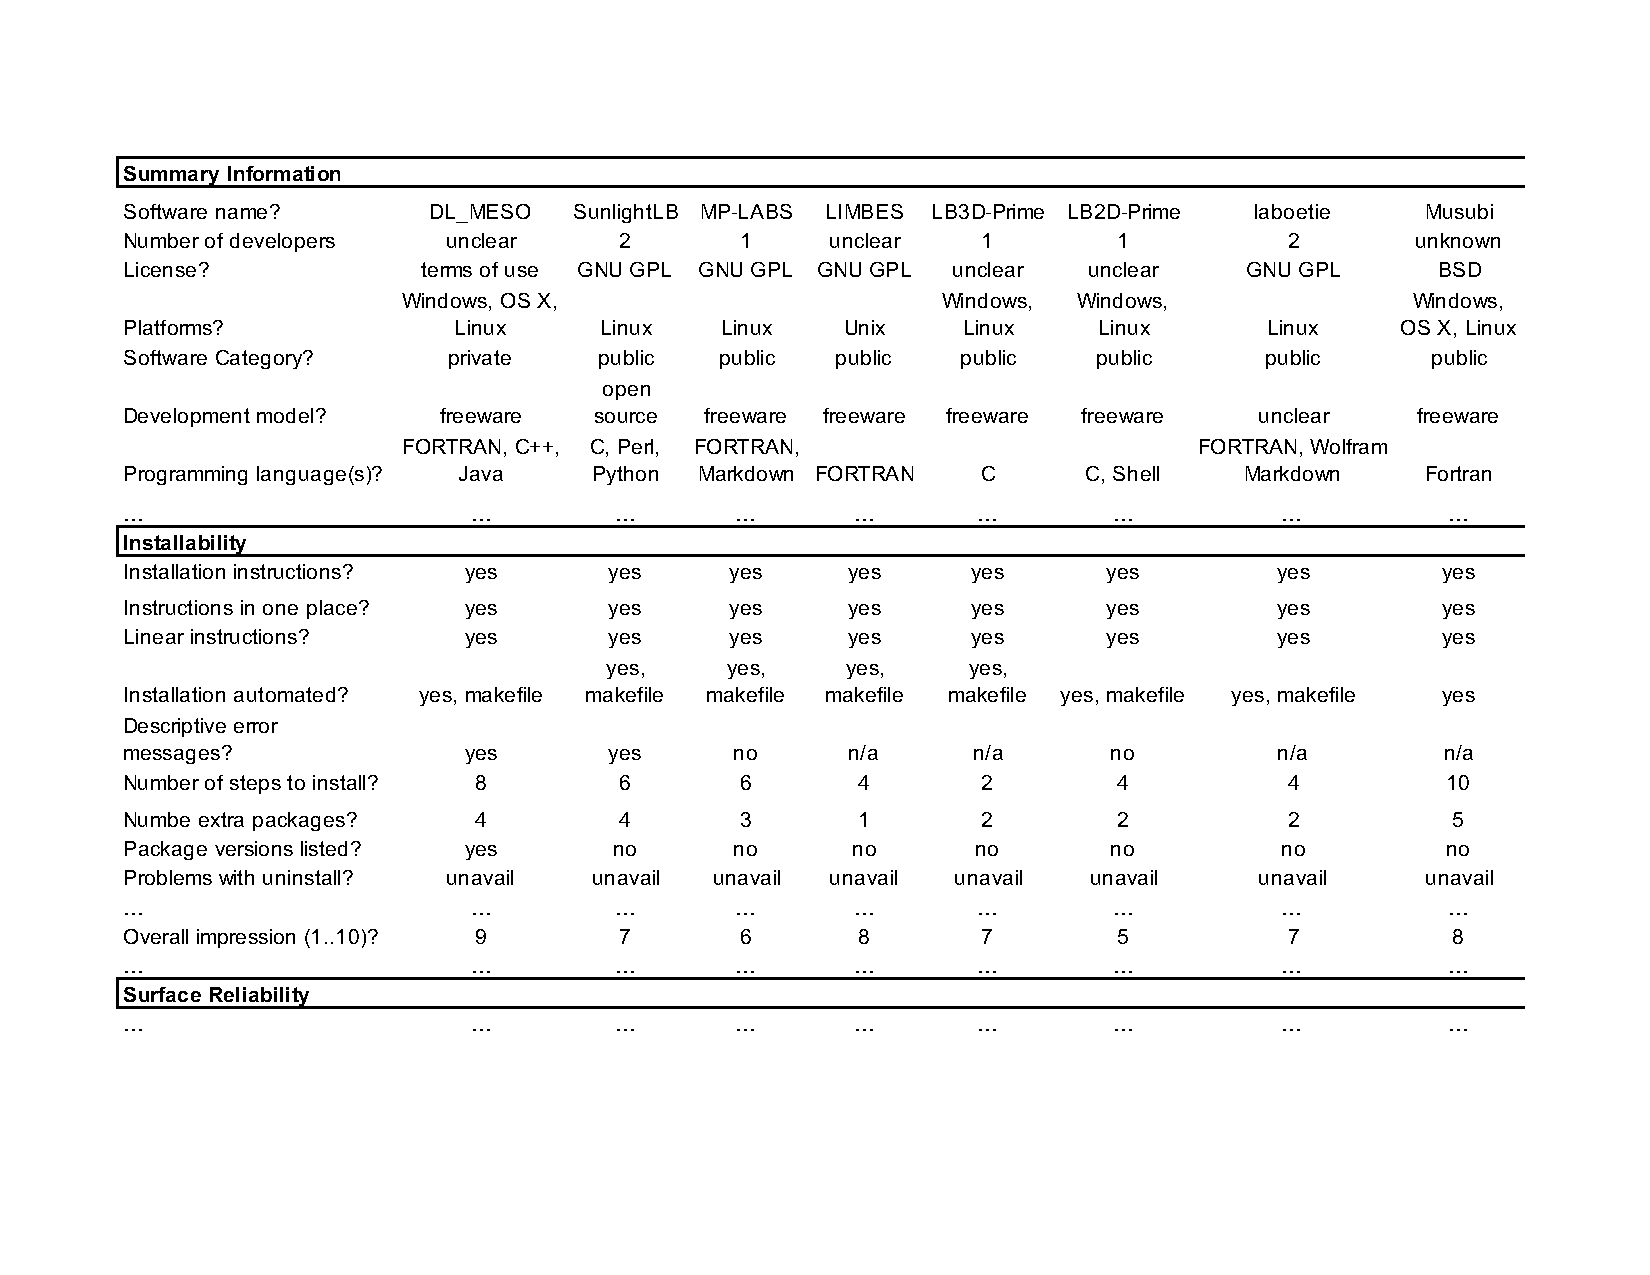
\includegraphics[width=1.0\textwidth]{./figures/measurement_template.pdf}
	  \caption{Excerpt of the Top Sections of the Measurement Template}
	  \label{measurement_template_image}
	\end{center}
\end{figure}

The full template consists of 108 questions categorized under 9 qualities:
\begin{inparaenum}[(i)]
	\item installability;
	\item correctness and verifiability;
	\item surface reliability;
	\item surface robustness;
	\item surface usability;
	\item maintainability;
	\item reusability;
	\item surface understandability; and,
	\item visibility/transparency. 
\end{inparaenum} 

The questions were designed to be unambiguous, quantifiable and measurable with
limited time and domain knowledge. The measures are grouped under headings for
each quality, and one for summary information
(Figure~\ref{measurement_template_image}).   The summary section provides
general information, such as the software name, number of developers, etc.  We
follow the definitions given by \cite{gewaltig2012quality} for the software
categories.  Public means software intended for public use.  Private means
software aimed only at a specific group, while the concept category is used for
software written simply to demonstrate algorithms or concepts. The three
categories of development models are: open source, where source code is freely
available under an open source license; free-ware, where a binary or executable
is provided for free; and, commercial, where the user must pay for the software
product.  

Several of the qualities use the word ``surface''.  This is to highlight that,
for these qualities in particular, the best that we can do is a shallow measure.
For instance, we do not conduct experiments to measure usability. Instead, we
are looking for an indication that usability was considered by the developers by
looking for cues in the documentation, such as getting started instructions, a
user manual or documentation of expected user characteristics.

Most of the data to be collected should be straightforward from reviewing the
measurement template.  However, in a few cases extra guidance is necessary
to eliminate ambiguity, as follows:

\begin{enumerate}
\item Publications about the software: A list of publications can be found
  directly on the website of some software packages. For others use Google
  Scholar or a similar index.
\item To answer whether there evidence that performance was considered, search
  the software artifacts for any mention of speed, storage, throughput,
  performance optimization, parallelism, multi-core processing, or similar
  considerations. The search function on GitHub can help.
\item Evidence of a getting started tutorial may be found within another
  artifact, like the user manual.
\item To find evidence of continuous integration, search the software artifacts
  for any mention of continuous integration. The search function on GitHub can
  help.  In some cases, \texttt{yaml} files will provide a hint that continuous
  integration is employed.
\end{enumerate}

Tools were use to find some of the measurements, such as the number of files,
number of lines of code (LOC), percentage of issues that are closed, etc. The
tool \href{https://github.com/tomgi/git_stats}{GitStats} was used to measure
each software package's GitHub repository for the number of binary files, the
number of added and deleted lines, and the number of commits over varying time
intervals. The tool \href{https://github.com/boyter/scc}{Sloc Cloc and Code
(scc)} was used to measure the number of text based files as well as the number
of total, code, comment, and blank lines in each GitHub repository.

As in \cite{SmithEtAl2016}, Virtual machines (VMs) are used to provide an
optimal testing environments for each package. VMs were used because it is
easier to start with a fresh environment without having to worry about existing
libraries and conflicts. Moreover, when the tests are complete the VM can be
deleted, without any impact on the host operating system. The most significant
advantage of using VMs is to level the playing field. Every software install
starts from a clean slate, which removes ``works-on-my-computer'' errors.

\subsection{Analytical Hierarchy Process} \label{AHP}

Once we have measured each package, we still need to rank them to answer
\rqref{RQ_HighestQuality}.  To do this, we used the Analytical Hierarchy Process
(AHP), a decision-making technique that is used to compare multiple options by
multiple criteria \cite{Saaty}. AHP performs a pairwise analysis using a matrix
and generates an overall score as well as individual quality scores for each
software package. The advantage of pair-wise comparisons is that they
facilitates a separation of concerns.  Rather than worry about the entire
problem, the decision maker can focus on one comparison at a time.  In our work
AHP is used for comparing and ranking the software packages of a domain using
the quality scores that are gathered in the Measurement Template
(Appendix~\ref{SecGradingTemplate}). AHP performs a pairwise analysis between
each of the 9 quality options for each of the 30 software packages.  This
results in a matrix, which is used to generate an overall score for each
software package for the given criteria. \cite{SmithEtAl2016} shows how AHP is
applied to ranking software based on quality measures.

Example of LBM measurement - maybe show the summary of all qualities?

\subsection{Interview Developers} \label{SecSurvey}

Several of the research question (\rqref{RQ_CompareToolsProjMngmnt},
\rqref{RQ_CompareMethodologies}, \rqref{RQ_PainPoints}, \rqref{RQ_Concerns} and
\rqref{RQ_Recommend}) require going beyond the quantitative data from the
measurement template. To gain the required insight, we interview developers
using a list of 20 questions \cite{SmithEtAl2021}. The questions cover the
background of the development teams, the interviewees, and the software itself.
We ask the developers how they organize their projects. We also ask them about
their understanding of the users. Some questions focus on the current and past
difficulties, and the solutions the team has found, or will try. We also discuss
the importance of, and the current situation for, documentation. A few questions
are about specific software qualities, such as maintainability,
understandability, usability, and reproducibility. The interviews are
semi-structured based on the question list; we ask follow-up questions when
necessary.  Each interview takes an 1 hour on average.

Our methodology suggests requesting interviews with a developer from each of the
30 software package.  Requests for interviews are sent to all packages so as to
not cause a potential bias by singling out any subset of the list. Moreover,
since not every developer will agree to the interview request, asking 30 times
will typically yield a reasonable number of responses. In our experience, the
response rate is between 15\% and 30\%.  In some cases multiple developers from
the same project will agree to be interviewed. When sending out interview
requests, we recommend finding the contacts on the projects’ website, or code
repository, or publications, or the biographic pages of the teams’ institutions.
We send at most two interview request emails to a contact for each software
package.  Meeting will typically be held using on-line meeting software, like
Zoom or Teams, facilitates recording and automatic transcription of the
meetings.

The interviewees should follow a process where they can make informed consent.
The interviews should follow standard ethics guideline of asking for consent
before interviewing, recording, and including participant details in the report.
The interview process presented here was approved by the McMaster University
Research Ethics Board under the application number 
\href{https://github.com/smiths/AIMSS/blob/master/StateOfPractice/MACREM/Application.pdf}
{MREB\#: 5219}.

For LBM we were able to recruit 4 developers to participate in our study.
Results in next sections.

\subsection{Interaction With Domain Expert} \label{sec_vet_software_list}

We partnered with a Domain Expert to vet our list of projects
(\rqref{RQ_WhatProjects}) and our ranking (\rqref{RQ_HighestQuality}).  The
Domain Expert is an important member of the state of the practice assessment
team. Pitfalls exist if non-experts attempt to acquire an authoritative list of
software, or try to definitively rank the software. Non-experts have the problem
that they can only rely on information available on-line, which has the
following drawbacks:
\begin{inparaenum}[i)]
  \item the on-line resources could have false or inaccurate information; and,
  \item the on-line resources could leave out relevant information that is so
in-grained with experts that nobody thinks to explicitly record it.
\end{inparaenum}

Domain experts may be recruited from academia or industry.  The only
requirements are knowledge of the domain and a willingness to be engaged in the
assessment process.  The Domain Expert does not have to be a software developer,
but they should be a user of domain software.  Given that the domain experts are
likely to be busy people, the measurement process cannot put to much of a burden
on their time.

The Domain Expert has an important role with verifying the list of LBM packages.
In advance of the first meeting with the Domain Expert, they were asked to
create a list of top software packages in the domain.  This is done to help the
expert get in the right mind set in advance of the meeting.  Moreover, by doing
the exercise in advance, we avoid the potential pitfall of the expert approving
the discovered list of software without giving it adequate thought.  The Domain
Expert was also asked to vet the collected data and analysis.  In particular,
they were asked to vet the proposed list of software packages and the AHP
ranking.

For the LBM project, our Domain Expert was Dr.\
Zahra Motamed, Assistant Professor of Mechanical Engineering at McMaster
University, Hamilton, Ontario, Canada.  

\subsection{Domain Analysis} \label{SecDomainAnalysis}

Since each domain we will study will have a reasonably small scope, we will be
able to view the software as constituting a program family.  The concept of a
program family is defined by \cite{parnas1976design} as ``a set of programs
whose common properties are so extensive that it is advantageous to study the
common properties of the programs before analyzing individual members''.
Studying the common properties within a family of related programs is termed a
domain analysis.  For the current methodology time constraints necessitate a
shallow domain analysis.  A table should be constructed that distinguishes the
programs under study by the variabilities that distinguish them.  In research
software the variabilities are often related to assumptions.  Table~\ref{} shows
the variabilities for the LBM software example.

\section{Comparison to Community Ranking} \label{repmetrics}

To address \rqref{RQ_CompareHQ2Popular} we need to compare the ranking by best
practices to the communities ranking.  Our best practices ranking comes from the
results of the AHP ranking (Section~\ref{AHP}).  We estimate the communities
ranking by repository stars and watches.  The comparison will provide insight on
whether best practices are rewarded by popularity.  However, inconsistencies
between the AHP ranking and the communities ranking are in inevitable for the
following reasons: 
\begin{inparaenum}[i)]
	\item the overall quality ranking via AHP makes the unrealistic assumption
	of equal weighting between the different quality factors;
	\item stars are known to not be a particularly good measure of popularity,
	since young projects have less time to accumulate stars \cite{}; 
	\item and, as for consumer products, there are more factors that determine
	popularity than quality alone.
\end{inparaenum}

Table~\ref{repometrics} compares the AHP ranking of the LBM package versus their
popularity in the research community.  Nine packages do not use GitHub, so they
do not have a measure of repository stars. Looking at the repository stars of
the other 15 packages, we can observe a pattern where packages that have been
highly ranked by our assessment tend to have more stars than lower ranked
packages. The best ranked package by AHP (ESPResSo) has the second most stars,
while the ninth ranked package (Sailfish) has the highest number of stars. The
same correlation is observed in the repository watch column, although this
column contains less data, since two of the packages (Palabos, waLBerla) use
GitLab, which does not track watches. Packages designated as lower quality often
do not use GitHub or GitLab, or have only a few stars/watches. Although the AHP
ranking and the community popularity estimate are not perfect measures, they do
suggest a correlation between best practices and popularity. We do not know
which comes first, the use of best practices or popularity, but we do know that
the top ranked packages tend to incorporate best practices.

\begin{table}[!h]
	\begin{center}
		\begin{tabular}{ p{3cm}p{1.25cm}p{1.75cm}p{1.75cm}p{1.75cm}p{1.75cm} }
			\toprule
			Name & Our Ranking & Repository Stars & Repository Star Rank &
			Repository Watches & Repository Watch Rank\\
			\midrule
			ESPResSo & 1 & 145 & 2 & 19& 2\\
			Ludwig & 2 & 27 & 8 & 6& 7\\
			Palabos & 3 & 34 & 6 & GitLab& GitLab\\
			OpenLB & 4 & No Git & No Git & No Git& No Git\\
			LUMA & 5 & 33 & 7 & 12& 4\\
			pyLBM & 6 & 95 & 3 & 10& 5\\
			DL\_MESO (LBE) & 7 & No Git & No Git & No Git & No Git\\
			Musubi & 8 & No Git & No Git & No Git & No Git\\
			Sailfish & 9 & 186 & 1 & 41& 1\\
			waLBerla & 10 & 20 & 9 & GitLab& GitLab\\
			laboetie & 11 & 4 & 13 & 5& 8\\
			TCLB & 12 & 95 & 3 & 16& 3\\
			MechSys & 13 & No Git & No Git & No Git& No Git\\
			lettuce & 14 & 48 & 4 & 5& 8\\
			ESPResSo++ & 15 & 35 & 5 & 12& 4\\
			MP-LABS & 16 & 12 & 11 & 2& 9\\			
			SunlightLB & 17 & No Git & No Git & No Git& No Git\\
			LB3D & 18 & No Git & No Git & No Git& No Git\\			
			LIMBES & 19 & No Git & No Git & No Git& No Git\\
			LB2D-Prime & 20 & No Git & No Git & No Git& No Git\\		
			HemeLB & 21 & 12 & 11 & 12& 4\\
			lbmpy & 22 &  11 & 12 & 2& 9\\	
			LB3D-Prime & 23 & No Git & No Git & No Git& No Git\\	
			LatBo.jl & 24 & 17 & 10 & 8& 6\\			
			\bottomrule
		\end{tabular}
		\caption{Repository Ranking Metrics} \label{repometrics}
	\end{center}
	\end{table}

\section{Comparison Between LBM and Research Software for Artifacts}
\label{Sec_CompareArtifacts}

In this step of the methodology we answer \rqref{RQ_CompareArtifacts} by
comparing the artifacts that we observed in LBM repositories to those observed
and recommended for research software in general.  As part of filling in the
measurement template (Section~\ref{}), the domain software is examined for the
presence of artifacts, which are then categorized by frequency. We suggest
grouping them into the categories: common, less common, and rare.  Common
artifacts are those found in more than two thirds of the examples, less common
artifacts are between 1/3 and 2/3, while rare are in less than 1/3 of the
software packages.  

The observed frequency of artifacts should then be compared to the artifacts
recommended by research software guidelines.  Table~\ref{} summarizes the
artifacts recommended by some existing guidelines.  

\begin{table}[!h]
\begin{center}
\begin{tabular}{ p{3cm}p{1cm}p{1cm}p{1cm}p{1cm}p{1cm}p{1cm}p{1cm}p{1cm}p{1cm} }
\toprule
~ \ & \cite{USGS2019} & \cite{TobiasEtAl2018} & \cite{BrettEtAl2021} & \cite{WilsonEtAl2016} & \cite{SmithAndRoscoe2018} & \cite{HerouxEtAl2008} & \cite{ThielEtAl2020} & \cite{vanGompelEtAl2016} & \cite{OrvizEtAl2017}\\
\midrule
LICENSE & \checkmark &  & \checkmark & \checkmark & \checkmark & & \checkmark & \checkmark & \checkmark\\
README &  &  &  &  & & & & \\
CONTRIBUTING &  &  &  &  & & & & & \\
CITATION &  &  &  &  & & & & & \\
CHANGELOG &  &  &  &  & & & & & \\
INSTALL &  &  &  &  & & & & & \\
Uninstall &  &  &  &  & & & & & \\
Contributor Guide &  &  &  &  & & & & & \\
Getting started &  &  &  &  & & & & & \\
User manual &  &  &  &  & & & & & \\
Tutorials &  &  &  &  & & & & & \\
FAQ &  &  &  &  & & & & & \\
Dependency List &  &  &  & & & & & & \\
Issue Track &  &  &  &  & & & & & \\
Version Control &  &  &  &  & & & & &\\ 
Requirements &  &  &  &  & & & & & \\
Design &  &  &  &  & & & & & \\
API Doc. &  &  &  &  & & & & & \\
Build Scripts &  &  &  &  & & & & & \\
Unit Tests &  &  &  &  & & & & & \\
Test Plan &  &  &  &  & & & & & \\
Integ. Tests &  &  &  &  & & & & &  \\
System Tests &  &  &  &  & & & & & \\
Acceptance Tests &  &  &  &  & & & & &  \\
Regression Tests &  &  &  &  & & & & & \\
Code Style Guide &  &  &  &  & & & & & \\
Release Info. &  &  &  &  & & & & & \\
Product Roadmap &  &  &  &  & & & & & \\
Code of Conduct &  &  &  &  & & & & & \\
\midrule
\end{tabular}
\caption{Commonly Recommended Artifacts in Software Development Guidelines} \label{Tbl_Guidelines}
\end{center}
\end{table}

The results for the LBM example are shown in Table~\ref{artifactspresent}.  The
majority of LBM generated artifacts correspond to general recommendations from
research software developers.  A union of the three columns in
Table~\ref{artifactspresent} mostly corresponds to recommendations made by the
research software community, as shown in Table~\ref{Tbl_Guidelines}.

\begin{table}
\begin{center}
\begin{tabular}{ p{12 cm}}
%\toprule
\textbf{Common}\\
\midrule
Developer List, Issue Tracker, Dependency List, Installation Guide, Theory
Notes, Related Publications, Build Files, README File, License, Tutorial,
Version Control\\
%\midrule
\textbf{Less Common}\\
\midrule
Change Log, Design Doc., Functional Spec., Performance Info., Test Cases, User
Manual\\
%\midrule
\textbf{Rare}\\
\midrule
API Doc., Developer Manual, FAQ, Verification Plan, Video Guide, Requirements
Spec.\\
%\bottomrule
\end{tabular}
\caption{Artifacts Present in LBM Packages, Classified by Frequency}
\label{artifactspresent}
\end{center}
\end{table}

Although the LBM community participates in most of the practices we found listed
in the general research software guidelines, some recommended practices were not
observed or rarely observed. For instance API documentation was rarely observed
for LBM software, but it is a frequently recommended (Table~\ref{Tbl_Guidelines}).
In addition to the items in the last column of Table~\ref{artifactspresent}, we
can add the following community recommended items that we rarely, if ever,
observed:

\begin{itemize}
\item A roadmap showing what is planned for the future.
\item A code of conduct to explicitly say how developers should treat one
another.
\item Programming style guidelines so that programming labels and formatting are
consistent \cite{TobiasEtAl2018,ThielEtAl2020,OrvizEtAl2017,Zadka2018,vanGompelEtAl2016,WilsonEtAl2014}.  We saw this information as part of
some developer guides, but only rarely.
\item Checklists can be used in projects to ensure that best practices are
followed by all developers.  Some examples include checklists merging branches
into master \cite{Brown2015}, checklists for saving and sharing changes to the
project \cite{WilsonEtAl2016}, checklists for new and departing team members
\cite{HerouxAndBernholdt2018}, checklists for processes related to commits and
releases \cite{HerouxEtAl2008} and checklists for overall software quality
\cite{ThielEtAl2020,SSI2022}.  For LBM software, ESPResSo has a checklist for
managing releases, but otherwise they are used only rarely for LBM.
\item Uninstall instructions \cite{vanGompelEtAl2016} were not observed for any
of the LBM projects.
\end{itemize}

\section{Comparison of Tool Usage Between LBM and Other Research Software}
\label{Sec_CompareTools}

Software tools are used to support the development, verification, maintenance,
and evolution of software, software processes, and artifacts \cite[p.\
501]{GhezziEtAl2003}. Many tools are used by LBM software packages, as
summarized in Table~\ref{tbl_tools}.  The tools are subdivided into development
tools, dependencies, and project management tools.  In this section we answer
\rqref{RQ_CompareToolsProjMngmnt} by comparing aspects of the tool usage in LBM
to their utilization in the research software community in general.

\begin{table}
\begin{center}
\begin{tabular}{ p{12 cm}}
%\toprule
\textbf{Development Tools}\\
\midrule
Continuous Integration, Code Editors, Development Environments, Runtime
Environments, Compilers, Unit Testing Tools, Correctness Verification Tools\\
%\midrule
\textbf{Dependencies}\\
\midrule
Build Automation Tools, Technical Libraries, Domain Specific Libraries\\
%\midrule
\textbf{Project Management Tools}\\
\midrule
Collaboration Tools, Email, Change Tracking Tools, Version Control Tools, Document Generation Tools\\
%\bottomrule
\end{tabular}
\caption{Observed development tools, dependencies and project management tools} 
\label{tbl_tools}
\end{center}
\end{table}
	
Development tools support the development of end products, but do not become
part of them, unlike dependencies that remain in the application once it is
released \cite[p.\ 506]{GhezziEtAl2003}. Although not shown in
Table~\ref{tbl_tools}, debuggers were also likely used.  Only three (ESPResSo,
Ludwig and Musubi) packages mentioned continuous integration tools, like Travis
CI. Code editors and compilers were explicitly noted to have been used by
several packages, and were likely used by all of them. One of the packages
(Ludwig) explicitly noted the use of proprietary unit testing code written in C.
Likewise, the use of proprietary code for verifying the correctness of output
was noted by one of the developers (pyLBM). Similar tools were likely used when
developing the other software packages.

For the dependency tools (Table~\ref{tbl_tools}), we observed that most of the
software packages use some sort of build automation tools, most commonly Make.
They all use various technical and domain specific libraries. Technical
libraries include visualization (e.g.\ Matplotlib, ParaView, Pygame, VTK), data
analysis (e.g.\ Anaconda, Torch), and message passing libraries (e.g.\ MPICH,
Open MPI, PyZMQ). Domain specific libraries include scientific computing
libraries (e.g.\ SciPy).

Many of the software packages that were assessed were developed by teams of two
or more people. Their work needed to be coordinated and managed.
Table~\ref{tbl_tools} shows the types of project management tools that were
explicitly noted in the artifacts, web-pages, or interviews with the developers.
As with development tools and dependencies, it is possible that other types of
project management tools are used, but they were not visible in the artifacts to
which we had access.  Collaboration tools, most often email and video, are noted
as being used when developing the software projects. Project management software
was not explicitly mentioned, but it is possible that some of the projects use
such software. Many of the projects are located on GitHub, where the developers
use the platform to help manage their projects, especially bug related issues.
Most of the projects appear to use change tracking and version control tools.
Document generation tools are mentioned in 12 of the 24 projects. The tools
Sphinx and Doxygen are explicitly used in this capacity.

The poor adoption of version control tools that Wilson lamented in 2006
\cite{Wilson2006} has greatly improved in the intervening years.  From
Section~\ref{Sec_Maintainability}, 67\% of LBM packages use version control
(GitHub, GitLab or CVS).  (From Table~\ref{gitrepodata}, 11/15 or 73\% of alive
packages use version control.)  The proliferation of version control tools for
LBM matches the increase in the broader research software community.  A little
over 10 years ago version control was estimated to be used in only 50\% of
research software projects \cite{Nguyen-HoanEtAl2010}, but even at that time
\cite{Nguyen-HoanEtAl2010} noted an increase from previous usage levels. A
survey in 2018 shows 81\% of developers use a version control system
\cite{AlNoamanyAndBorghi2018}.  \cite{Smith2018} has similar results, showing
version control usage for alive projects in mesh generation, geographic
information systems and statistical software for psychiatry increasing from
75\%, 89\% and 17\% (respectively) to 100\%, 95\% and 100\% (respectively) over
a four year period ending in 2018.  (For completeness the same study showed a
decrease in version control usage for seismology software over the same time
period, from 41\% down to 36\%).  Almost every software guide cited in
Section~\ref{Sec_CompareArtifacts} includes the advice to use version control.
The high usage of version control tools in LBM software matches the trend in
research software in general.

As mentioned in Section~\ref{SecSurfCorrectAndVerifiab}, continuous integration
is rarely used in LBM (3 of 24 packages or 12.5\%). This contrasts with the
frequency with which continuous integration is recommended in research software
development guidelines \cite{BrettEtAl2021,Brown2015,ThielEtAl2020,Zadka2018,vanGompelEtAl2016}.  We could not find published data on the
frequency with which continuous integration is used in general research
software.  Our impression is that like LBM software, other research software
packages lag behind the recommended best practice of employing continuous
integration tools.

Interviews with the developers revealed a potentially more frequent use of both
unit testing and continuous integration, compared to what was observed from
studying the repository artifacts.

\section{Comparison of Principles, Process and Methodologies to Research Software in General} \label{Sec_CompareMethodologies}

This section answers research question \rqref{RQ_CompareMethodologies} by
comparing the principles, processes and methodologies used for LBM software to
what can be gleaned from the literature on research software in general. In our
data collection for LBM software, the software development process is not
explicitly indicated in the artifacts for most of the packages. However, during
our interviews one developer (ESPResSo) told us their non-rigorous development
model is like a combination of agile and waterfall. Employing a loosely defined
process makes sense for LBM software, given that the teams are generally small
and self-contained.  Although eleven of the packages explicitly convey that they
would accept outside contributors, generally the teams are centralized, often
working at the same institution.  Working at the same institution means that an
informal process can show success, since informal conversations are relatively
easy to have.

Interviews with developers confirmed a similar project management processes. In
teams of only a couple of developers, additions of new features or major changes
are discussed with the entire team. Projects with more than a couple developers
have lead developer roles. These lead developers review potential additions to
the software. One of the developers (ESPResSo) that was interviewed noted that
an ad hoc peer review process is used to assess major changes and additions.
Using peer review (also called technical review) matches with recommended
practice for research software \cite{HerouxEtAl2008,Givler2020,OrvizEtAl2017,USGS2019}.

Two types of software changes were discussed during interviews with developers.
One is feature additions, which arise from a scientific or functional need.
These changes involve formal discussions within the development team, and lead
developer participation is mandatory. The other change type is code refactoring,
which only sometimes involves formal discussions with the development team. New
developers were noted to play an increased role in these changes compared to the
former changes. Software bugs are typically addressed in a similar fashion as
code refactoring.  Issue tracking is commonly used to manage these changes.

Our observations of a informally defined process, with elements of agile
methods, matches what has been observed for research software in general.
Scientific developers naturally use an agile philosophy \cite{AckroydEtAl2008,CarverEtAl2007,EasterbrookAndJohns2009,Segal2005,HeatonAndCarver2015}, or an
amethododical process \cite{Kelly2013}, or a knowledge acquisition driven
process \cite{Kelly2015}.

Most of the software packages do not explicitly state the motivations or design
principles that were considered when developing the software. One package,
Sailfish, indicates in its artifacts that shortening the development time was
considered in early stages of design, with the developers using Python and
CUDA/OpenCL to achieve this without sacrificing performance. The Sailfish goals
are explicitly listed as performance, scalability, agility and extendability,
maintenance, and ease of use. The project scored well in these categories during
our assessment.  The quality priorities for Sailfish roughly match the
priorities observed for research software in general.
\cite{Nguyen-HoanEtAl2010} surveyed developers to find the following list of
qualities, in decreasing order of importance: reliability, functionality,
maintainability, availability, performance, flexibility, testability, usability,
reusability, traceability, and portability. The Sailfish list does not list
reliability or functionality, but we can safely assume those are implicitly high
priorities for any scientific project.  In earlier studies
\cite{KellyAndSanders2008} and \cite{CarverEtAl2007} both highlight how
important correctness is for research software.

During our interviews, documentation was noted as playing a significant role in
the development process, specifically with on-boarding new developers. A goal of
documentation is to lower the entry barrier for these new contributors. The
documentation provides information on how to get started, orients the user to
artifacts and the source code, and explains how the system works, including the
so-called simulation engine and interface.  This emphasis on documentation,
especially for new developers, is echoed in research software guidelines.
Multiple guidelines recommend a document explaining how to contribute to a
project, often named CONTRIBUTING \cite{Yo2021,BrettEtAl2021,WilsonEtAl2016,ThielEtAl2020,vanGompelEtAl2016,OrvizEtAl2017,FLOSS2022,JimenezEtAl2017}.
Tutorials \cite{ThielEtAl2020}, trouble shooting guides \cite{OrvizEtAl2017,SSI2022} and quick start examples \cite{ThielEtAl2020,vanGompelEtAl2016} are
also recommended.  \cite{SmithAndRoscoe2018} suggests including instructions
specifically for on-boarding new developers. For open source software in general
(not just research software), \cite{Fogel2005} recommends providing tutorial
style examples, developer guidelines, demos and screenshots.

\section{Developer Pain Points} \label{painpoints}

Based on interviews with 4 developers, this section aims to answer the research
questions: i) What are the pain points for developers working on research
software projects (\rqref{RQ_PainPoints})?; and, ii) How do the pain points of
developers from LBM compare to the pain points for research software in general
(\rqref{RQ_ComparePainPoints})?  Below we go through each of the identified pain
points and include citations that contrast the LBM experience with observations
from researchers in other domains.  Potential ways to address the pain points
are covered in Section~\ref{Sec_AddressConcerns}. The full interview questions
are found in \cite{SmithEtAl2021}.

\cite{PintoEtAl2018} lists some pain points that did not come up in our
conversations with LBM developers: Cross-platform compatibility, interruptions
while coding, scope bloat, lack of user feedback, hard to collaborate on
software projects, and aloneness. \cite{WieseEtAl2019} repeat some of the
previous pain points and add the following: dependency management, data handling
concerns (like data quality, data management and data privacy), reproducibility,
and software scope determination. Although LBM developers did not mention these
pain points, we cannot conclude that they are not relevant for LBM software
development, since we only interviewed 4 LBM developers for about an hour each.

\begin{enumerate}

	\item[P\refstepcounter{pnum}\thepnum \label{P_LackDevTime}:] \textbf{Lack of
	Development Time} A developer of pyLBM noted that their small development
	team has a lack of time to implement new features. Small development teams
	are common for LBM software packages (as shown in the measurement table
	excerpt in Figure~\ref{measurement_template_image}). Lack of time is also
	highlighted as a pain point by other research software developers
	\cite{PintoEtAl2018,PintoEtAl2016,WieseEtAl2019}.

	\item[P\refstepcounter{pnum}\thepnum \label{P_LackSoftDevExp}:] \textbf{Lack
	of Software Development Experience} A lack of software development
	experience was noted by the developer of TCLB, and others noted a need for
	improving software engineering education. Many of the team members on their
	project are domain experts, not computer scientists or software engineers.
	This same trend is noted by \cite{Nguyen-HoanEtAl2010}, which showed only
	23\% of research software survey respondents having a computing-related
	background. Similarly, \cite{UditAndKatz2017} show that the majority (54\%)
	of postdocs have not received training in software development.  The LBM
	developer suggesting an increasing role for formal software education
	matches the trend observed by \cite{PintoEtAl2018}, where their replication
	of a previous study \cite{HannayEtAl2009}, shows a growing interest in
	formal training (From 13\% of respondents in 2009 to 22\% in 2018).
	\cite{PintoEtAl2018} found that some developers feel there is a mismatch
	between coding skills and subject-matter skills. 
	
	\item[P\refstepcounter{pnum}\thepnum \label{P_LackFunding}:] \textbf{Lack of
	Incentive and Funding} The TCLB developer noted a lack of incentives and
	funding in academia for developing widely used scientific software. This
	problem has also been noted others \cite{gewaltig2012quality,Goble2014,KaterbowAndFeulner2018}.  \cite{WieseEtAl2019} reported developer pains
	related to publicity, since historically publishing norms make it difficult
	to get credit for creating software.  As studied by
	\cite{HowisonAndBullard2016}, research software (specifically biology
	software, but the trend likely applies to other research software domains)
	is infrequently cited.  \cite{PintoEtAl2018} also mentions the lack of
	formal reward system for research software.

	\item[P\refstepcounter{pnum}\thepnum \label{P_LackExtSupport}:] \textbf{Lack
	of External Support} A concern was raised that there are no organizations
	helping with the development of good quality software.  This concern is not
	echoed in the literature because there are such organizations, including
	\href{https://bssw.io/} {Better Scientific Software (BSSw)},
	\href{https://www.software.ac.uk/} {Software Sustainability Institute}
	\cite{CrouchEtAl2013}, and \href{https://software-carpentry.org/}{Software
	Carpentry} [* {WilsonAndLumsdaine2006, Wilson2016} *]. Over time awareness of
	these groups will grow, so this pain point is likely to disappear in the
	future for LBM and other research software developers.
		
	\item[P\refstepcounter{pnum}\thepnum \label{P_TechnologyHurdles}:]
	\textbf{Technology Hurdles} Technology pain points include setting up
	parallelization and continuous integration.

	\item[P\refstepcounter{pnum}\thepnum \label{P_Correctness}:]
	\textbf{Ensuring Correctness} Difficulties with ensuring correctness were
	noted by several developers. Several developers alluded to difficulty with
	testing the correctness of large numbers of features, and some manually
	tested program output, as opposed to using automated testing. The TCLB
	developer commented that the amount of testing data needed was sometimes
	problematic, since free testing services do not offer adequate facilities
	for large amounts of data, which means in-house testing solutions are
	needed.  Other research software domains point to the following problems
	with testing: i) \cite{PintoEtAl2018} mention the problem of insufficient
	testing; ii) the survey of \cite{HannayEtAl2009} shows that more developers
	think testing is important than the number that believe they have a
	sufficient understanding of testing concepts; and, iii)
	\cite{HannayEtAl2009,KanewalaAndBieman2013,KellyEtAl2011,WieseEtAl2019}
	point to the oracle problem, which occurs in research software when we do
	not have a means to judge the correctness of the calculated solutions.  The
	LBM experience seems to overlap with i and ii, but the LBM developers did
	not allude to problem iii (the oracle problem) in our conversation; we
	believe that they have developed techniques to work around the oracle
	problem.  
	
	\item[P\refstepcounter{pnum}\thepnum \label{P_Usability}:]
	\textbf{Usability} Several developers noted that users sometimes try to use
	incorrect LBM method combinations to solve their problems. Furthermore, some
	users think that the packages will work out of the box to solve their cases,
	while in reality CFD knowledge needs to be applied to correctly modify the
	packages for the new endeavour.  \cite{WieseEtAl2019} also interacted with
	developers that mentioned that users do not always have the expertise
	required to install or use the software.
	
	\item[P\refstepcounter{pnum}\thepnum \label{P_TechDebt}:] \textbf{Technical
	Debt} The developer of ESPResSo said that their source code was written with
	a specific application in mind, which later caused too much coupling between
	components in the source code. This results in technical debt
	\cite{KruchtenEtAl2012}, which has an impact on future modifiability and
	reusability. Concern with technical debt is likely why researchers in the
	survey of \cite{Nguyen-HoanEtAl2010} rated maintainability as the third
	most important software quality. More recently the push for sustainable
	software \cite{deSouzaEtAl2019} is motivated by the pain that past
	developers have had with accumulating too much technical debt.

	\item[P\refstepcounter{pnum}\thepnum \label{P_Documentation}:]
	\textbf{Quality of Documentation}  The importance of documentation for both
	users and developers was stressed throughout the interviews. However, it was
	noted several times that a lack of time and funding (\ppref{P_LackDevTime})
	has a negative affect on the documentation. Most of the developers are
	scientific researchers evaluated on the scientific papers that they produce.
	Writing and updating documentation is something that is done in their free
	time, if that time arises. Inadequate research software documentation is
	also mentioned by others \cite{PintoEtAl2018,WieseEtAl2019} and the
	problem also arises with non-research software \cite{LethbridgeEtAl2003}.
	Recommendations on the development of research software state that
	developers should critically evaluate their own development processes in
	terms of quality assurance and comply with international standards for
	software documentation \cite{KaterbowAndFeulner2018}.

\end{enumerate}

\section{Lessons from LBM Developers} \label{Sec_AddressConcerns}

This section summarizes the best practices from LBM developers that are taken to
address the pain points mentioned in Section~\ref{painpoints}.  The main source
of information is the qualitative data from developer interviews
(Section~\ref{SecSurvey}).  The practices summarized in this section can
potentially be emulated by the LBM software packages that do not currently
follow them.  Moreover, these practices may also provide examples that can be
followed by other research software domains.

\subsection{Design For Change} \label{Sec_DesForChange}

Increasing source code modularity, reducing duplicate information,
and improving abstraction by developing well defined interfaces. This was noted
by the developers of ESPResSo and pyLBM.  A developer of pyLBM mentioned that
the geometries and models of their system had been ``decoupled'', using
abstraction and modularization of the source code, to make it ``very easy to add
[new] features''.  [*{Highlights the advantage of design.  Other projects can
look to these examples.  Maybe cite the Anshu paper about Flash? Dune? and point
to the advantages of design.}*] Addresses maintainability.  The developer of TCLB
mentioned that their package had two sets of code, for executing the models on
the CPU and GPU, and that maintenance was decreased by introducing macros, a
practice which became a common part of the development process. 

A high degree of code modularity and abstraction was noted by developers as a
measure to ensure the ease of future changes. This can be ensured by separating
components and hiding information behind well defined interfaces. The developer
of ESPResSo also noted that some of the code base was transitioned from C to
C++, which could ease modifiability of that software package. The developer of
TCLB noted that their software package was designed to allow for the addition of
some LBM features, but changes to major aspects of the system would be
difficult. For example, ``implementing a new model will be an easy
contribution'', but changes to the ``Cartesian mesh...will be a nightmare''.
[*{example suggests identifying likely changes.}*]

Modularize the source code, separate components, hide information behind well
defined interfaces. This is suggested in SCS literature, and in developer
comments.  [*{one of Wilson's best practices.}*]

\begin{itemize}
	\item Modifiability. Consider flexibility of data structures and data
	storage in the design stage. The package pyLBM redeveloped data structures
	to ease future changes.
	\item Reusability. Provide API documentation, if applicable. Only one
	(ESPResSo) of the top five ranked packages provided API documentation.
\end{itemize}

\section{Recommendations for Future Practices} \label{Sec_Recommendations}

Answers \rqref{RQ_Recommend}.  practices for the future.  Probably the easiest
approach is to list the practice and then the PPs that it helps.  Our
recommendations are not lists of what should have been done in the past, or what
should be done now; they are just suggestions for consideration in the future.

``unique challenges of scientific research (e.g., the frequent and unforeseen
changes in requirements ...)'' \cite{PintoEtAl2018}. We can point out that in
the future this viewpoint could change and why.  Not really a unique challenge.
Cite Smith 2016?

linters \cite{Zadka2018} were rarely observed in LBM projects.  Do not see much
evidence of their presence in best practice guides.

[*{Address lack of development time (\ppref{P_LackDevTime}): Aside from
on-boarding new developers, time constraints could be mitigated by increasing
developer efficiency, which could be addressed in several ways, including by
improving the quality of documentation, or incorporating automatic code
generation.} 

[*{Address lack of funding (\ppref{P_LackFunding}): The developer further
commented that there are no journals that publish such scientific software
source code. However, there are ways to get such source code cited. Work has
been done to address this in \cite{SmithEtAl2016-softcite}, which presents a
set of software citation principles and discusses ``how they could be used to
implement software citation in the scholarly community''
\cite{katz2019software}. other papers also mention this pain point.
Solutions proposed by Katz, journal of open source etc. Journal of Open Source
Software \cite{SmithEtAl2018-joss}.  Calling for direct software citations
\cite{SmithEtAl2016-softcite}.  Guidance on software citation from
\cite{KatzEtAl2021}.  Discussed in CarverEtAl2021 paper.}

[*{Address quality of documentation (\ppref{P_Documentation}): Make required
background of users explicit, possibly in a requirements document.}

Surface Correctness and Verifiability. Use a requirements
specification document. This is suggested in SCS literature, and several of
the top ranked packages had such a document or reference to theory manuals.
A potential template is presented in \cite{smith2005new}. 

Papers that talk about how to do open source.

Requirements documentation is feasible, as shown by the prevalence of theory
documents in LBM software.  Table~\ref{artifactspresent} shows that theory
documentation is common.  We observed 17 of 24 packages had at least some theory
documentation. Templates for scientific requirements, like
\cite{SmithEtAl2007,SmithAndLai2005}, show theory is a significant part of the
requirements documentation. With the addition of some extra information, the
theory documents can be transformed into requirements specification.  The key
extra information includes explicitly stating user characteristics, explicitly
stating how the user interacts with the software in terms of input data
requirements, and listing likely and unlikely changes.  Explicit statements
about likely changes are invaluable in the design stage, since they provide
developers guidance on how general the software needs to be.  For those wishing
to maximize the value of a requirement specification, information could be added
like prioritizing the nonfunctional requirements (to show the relative
importance between qualities like portability, reliability and performance) and
traceability information (to show the consequences of any changes to the
assumptions).

\section{Threats To Validity} \label{threats}

This section examines potential threats to the validity of this state of the
practice assessment. These can be categorized into methodology and data
collection issues. The goal of this assessment isn't to rank the software, but
to use the ranking exercise as a means to understand the state of the practice
of LBM software development.

The measures listed in our measurement template may not be broad enough to
accurately capture some qualities. For example, there are only two measures of
surface robustness. The measurement of robustness could be expanded, as it
currently only measures unexpected input. Other faults could be introduced, but
could require a large investment of time to develop, and might not be a fair
measure for all packages. Similarly, reusability is assessed along the number of
code files and LOC per file. While this measure is indicative of modularity, it
is possible that some packages have many files, with few LOC, but the files do
not contain source code that is easily reusable. The files may be poorly
formatted, or the source code may be vague and have ambiguous identifiers.
Furthermore, the measurement of understandability relies on 10 random source
code files. It is possible that the 10 files that were chosen to represent a
software package may not be a good representation of the understandability of
that package.

Regarding data collection, a risk to the validity of this assessment is missing
or incorrect data. Some software package data may not have been measured due to
technology issues like broken links. This issue arose with the measurement of
Palabos, which had a broken link to its user manual, as noted in
Section~\ref{Sec_CompareArtifacts}. 

Some pertinent data may not have been specified in public artifacts, or may be
obscure within an artifact or web-page. The use of unit testing and continuous
integration was mentioned in the artifacts of only three (ESPResSo, Ludwig,
Musubi) packages. However, interviews suggested a more frequent use of both unit
testing and continuous integration in the development processes than what was
observed from the initial survey of the artifacts. For example, OpenLB, pyLBM,
and TCLB use such methods during development despite this not being explicitly
clear from an analysis of the material available online. 

Furthermore, design documentation was measured to be a ``less common'' artifact
in this assessment, but it is probable that such documentation is part of all
LBM packages. After all, developing SCS is not a trivial endeavour. It is likely
that many packages have such documentation but did not make it public, and due
to this the measured data is not a true reflection of software package quality.

[*{There are more threats to validity.  Brainstorm.  Watch for them while 
editing.  Look at Ao paper.}

Problems with the measurement of qualities:

\begin{itemize}
\item The assumption that more code files is an indicator of reusability
(Section~\ref{reusabilityresults}) may not be a valid assumption.
\item Understandability was measured using only 10 random files
(Section~\ref{Sec_SurfUnderstandability}).  This could be improved.
\end{itemize}

Overall ranking with equally weighted qualities isn't realistic
(Section~\ref{Sec_OverallQuality}).

Threat to validity - the gap between measures of everything else and Musubi
(Section~\ref{identifysoftware}), and then the gap between the manual measures
and the automated measures (Section~\ref{repmetrics}).

From Section~\ref{Sec_CompareTools}: ``Interviews with the developers revealed a
potentially more frequent use of both unit testing and continuous integration,
compared to what was observed from studying the repository artifacts.''

Interviews suggested a more frequent use of both unit testing and continuous
integration in the development processes than what was observed from the initial
survey. For example, OpenLB, pyLBM, and TCLB use such methods during
development, despite this not being explicitly clear from an analysis of the
material available online.  The correctness and verifiability of such packages
is not measured well using surface analysis.

\section{Concluding Remarks} \label{SecConcludingRemarks}

Our comparison may point out areas where some LBM software
packages fall short of current best practices. This is not intended to be a
criticism of any existing packages, especially since in practice not every
project needs to achieve the highest possible quality.  However, rather than
delve into the nuances of which software can justify compromising which
practices we will write our comparison under the ideal assumption that every
project has sufficient resources to match best practices.

For each domain we wish to highlight success stories that can be shared amongst
domain community, and with the broader research software community, while at the
same time watching for areas for potential future improvement.

We have outlined a methodology for assessing the state of the practice for any
given research software domain.  (Although the scope of the current work has been
on research software, there is little in the methodology that is specific to
research software, except for the interview question related to the quality of
reproducibility.)  When applying the methodology to a given domain, we provide a
means to answer the following questions:
\begin{inparaenum}[i)]
\item What artifacts (documents, code, test cases, etc.) are present?
\item What tools are used?
\item What principles, process and methodologies are used?
\item What are the pain points for developers?
\item What actions are used to improve qualities like maintainability and
reproducibility?
\item What specific actions are taken to achieve the qualities of usability,
traceability, modifiability, maintainability, correctness, understandability,
unambiguity, reproducibility and visibility/transparency?
\item How does software designated as high quality by this methodology compare
  with top rated software by the community?
\end{inparaenum} 

The methodology depends on the engagement of a Domain Expert.  The Domain
Expert's role is to ensure that the assessment is consistent with the culture of
the community of practitioners in the domain.  The Domain Expert also has an
important role to play with the domain analysis.  For each domain we 
conduct a domain analysis to look at the commonalities, variabilities and
parameters of variation, for the family of software in the domain.  The domain
analysis means that software can be compared not just based on its quality, but
also based on its functionality.

The methodology follows a systematic procedure that begins with identifying the
domain and ends with answering the research questions posed above.  In between
we collect an authoritative list of about 30 software packages.  For each
package in the list we fill in our measurement template.  The template consists
of repository related data (like number of open issues, number of lines of code,
etc.) and 108 measures/questions related to 9 qualities: installability,
correctness/verifiability, reliability, robustness, usability, maintainability,
reusability, understandability and visibility/transparency. Filling in the
template requires installing the software, running simple tests (like completing
the getting started instructions (if present)), and searching the code,
documentation and test files.

The data for each domain is used to rank the software package according to each
quality dimension using AHP.  The ranking is not intended to identify a single
best software package.  Instead the ranking is intended to provide insights on
the top set of software for each quality.  The top performers can be contrasted
with the lesser performers to gain insight into what practices in the domain are
working.  Deeper insight can be obtained by combining this data with the
interview data from asking each recruited developer 20 questions.

Combining the quantitative data from the measurement template with the interview
results, along with the domain experts knowledge, we can determine the current
state of the practice for domain X.  Using our methodology, spreadsheet
templates and AHP tool, we estimate (based on our experience with using the
process) the time to complete an assessment for a given domain at 173 person
hours.

With the wealth of data from assessing the state of practice for multiple
domains, the next step is a meta-analysis.  We would look at how the different
domains compare. What lessons from one domain could be applied in other domains?
What (if any) differences exist in the pain points between domains?  Are there
differences in the tools, processes, and documentation between domains?

The current methodology is constrained by limited resources.  A 4 hour cap on
the measurement time for each software package limits what can be assessed.
Within this limit, we can't measure some important qualities, like usability and
modifiability.  In the future, we propose a more time-consuming process that
would capture these other quality measures.  To improve the feasibility, the
more time consuming measurements would not have to be completed for all 30
packages. Instead, a short list could be identified using the output of the AHP
ranking to select the top projects, or to select a sample of interesting
projects across the quality spectrum.

\subsubsection{Acknowledgements} Please place your acknowledgments at
the end of the paper, preceded by an unnumbered run-in heading (i.e.
3rd-level heading).

%
% ---- Bibliography ----
%
% BibTeX users should specify bibliography style 'splncs04'.
% References will then be sorted and formatted in the correct style.
%
\bibliographystyle{splncs04}
\bibliography{DiggingDeeper}
%
% \begin{thebibliography}{8}
% \bibitem{ref_article1}
% Author, F.: Article title. Journal \textbf{2}(5), 99--110 (2016)

% \bibitem{ref_lncs1}
% Author, F., Author, S.: Title of a proceedings paper. In: Editor,
% F., Editor, S. (eds.) CONFERENCE 2016, LNCS, vol. 9999, pp. 1--13.
% Springer, Heidelberg (2016). \doi{10.10007/1234567890}

% \bibitem{ref_book1}
% Author, F., Author, S., Author, T.: Book title. 2nd edn. Publisher,
% Location (1999)

% \bibitem{ref_proc1}
% Author, A.-B.: Contribution title. In: 9th International Proceedings
% on Proceedings, pp. 1--2. Publisher, Location (2010)

% \bibitem{ref_url1}
% LNCS Homepage, \url{http://www.springer.com/lncs}. Last accessed 4
% Oct 2017
% \end{thebibliography}
\end{document}